%======================================================================
% CAPITULO 1: ONBOARDING E IDENTIDAD
%======================================================================

\chapter{Onboarding e Identidad}
\label{ch:onboarding}

Todo nodo en \sdc{} debe tener una identidad unica para garantizar la auditoria y trazabilidad de todas las operaciones. Este capitulo guia al usuario a traves del proceso de configuracion inicial y vinculacion del dispositivo al ecosistema.

\section{Configuracion de Identidad}
\label{sec:config-identidad}

Al iniciar la aplicacion por primera vez, el sistema presenta una pantalla de bienvenida que solicita la configuracion basica de identidad. Este paso es fundamental para el funcionamiento correcto de todas las caracteristicas de auditoria y seguridad.

\begin{figure}[H]
\centering
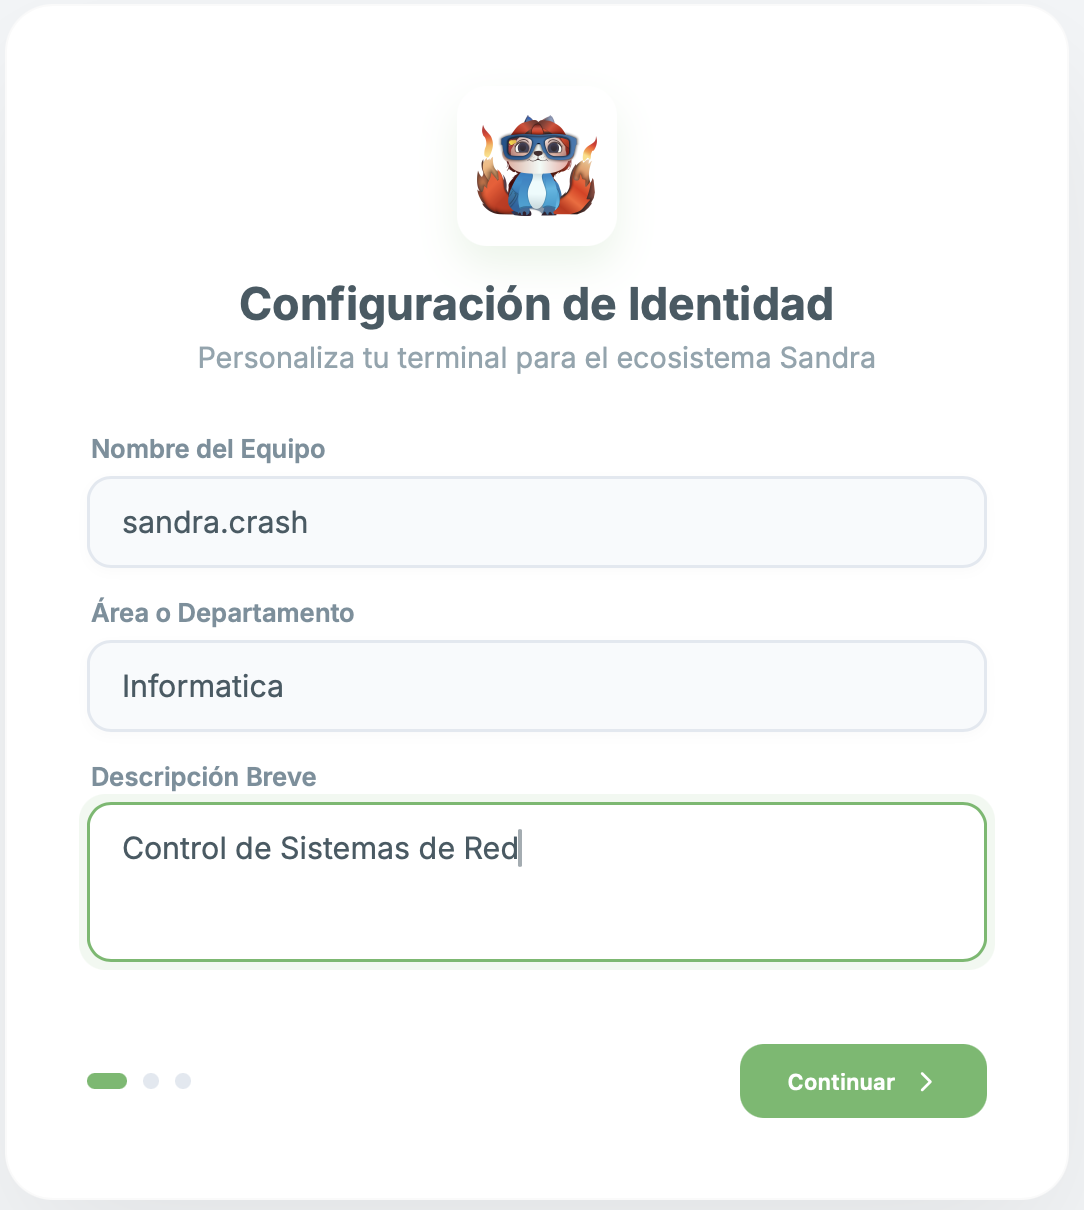
\includegraphics[width=0.5\textwidth]{anexos/2 config.png}
\caption{Pantalla de configuracion inicial de identidad}
\label{fig:config-inicial}
\end{figure}

\subsection{Campos de Configuracion}

La pantalla de configuracion inicial solicita la siguiente informacion:

\begin{table}[H]
\centering
\begin{tabular}{p{4cm}p{4cm}p{6cm}}
\toprule
\textbf{Campo} & \textbf{Ejemplo} & \textbf{Descripcion} \\
\midrule
Nombre del Equipo & sandra.crash & Identificador unico del nodo \\
Area & Desarrollo & Departamento o unidad organizativa \\
\bottomrule
\end{tabular}
\caption{Campos de configuracion de identidad}
\label{tab:campos-identidad}
\end{table}

\begin{quote}
\textbf{Importancia del Nombre del Equipo}\\
\small
Es vital asignar nombres descriptivos y consistentes con la nomenclatura de tu organizacion. Este nombre aparecera en todos los logs del Monitor de Sistema y sera utilizado para identificar el origen de las operaciones durante auditorias forenses.
\end{quote}

\subsection{Mejores Practicas para la Nomenclatura}

Se recomienda seguir estos patrones para los nombres de equipo:

\begin{itemize}[leftmargin=*]
    \item \textbf{Formato}: \texttt{[ambiente].[usuario]} o \texttt{[ubicacion].[funcion]}
    \item \textbf{Ejemplos validos}:
    \begin{itemize}
        \item \texttt{prod.server01} -- Servidor de produccion
        \item \texttt{dev.carlos} -- Estacion de desarrollo
        \item \texttt{hq.finanzas} -- Equipo de finanzas en sede principal
    \end{itemize}
    \item \textbf{Evitar}: espacios, caracteres especiales o nombres genericos como PC-1 o Equipo
\end{itemize}

\section{Vinculacion del Nodo}
\label{sec:vinculacion}

Una vez configurada la identidad basica, SDC procede a detectar automaticamente el entorno del dispositivo y generar un identificador unico de cliente (Client ID).

\begin{figure}[H]
\centering
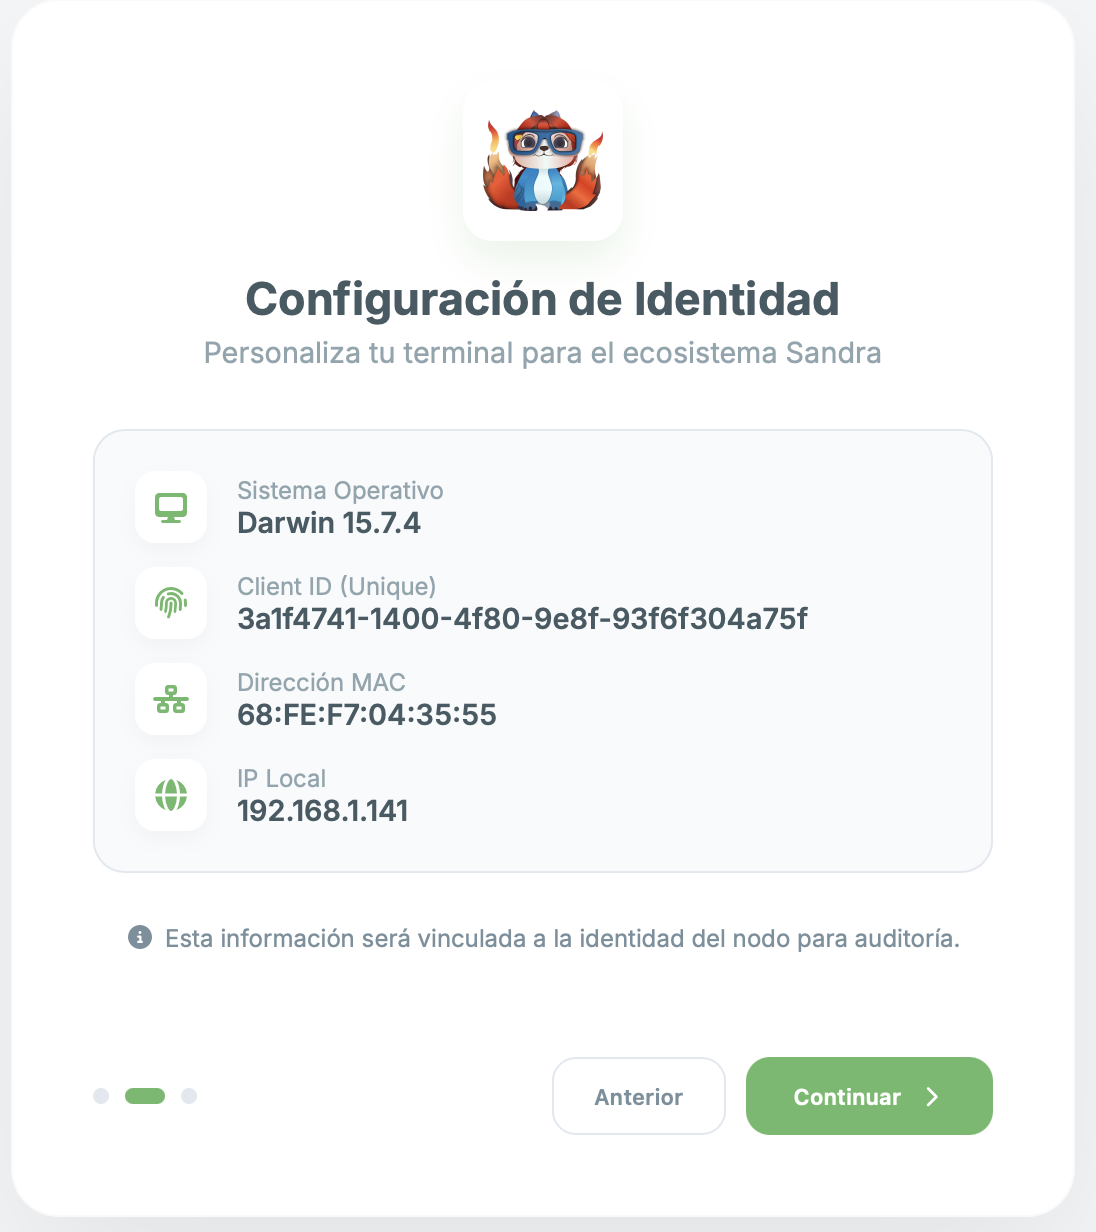
\includegraphics[width=0.5\textwidth]{anexos/3 config.png}
\caption{Pantalla de vinculacion y deteccion de entorno}
\label{fig:vinculacion}
\end{figure}

\subsection{Informacion Detectada Automaticamente}

\begin{table}[H]
\centering
\begin{tabular}{p{4cm}p{3cm}p{7cm}}
\toprule
\textbf{Parametro} & \textbf{Ejemplo} & \textbf{Uso} \\
\midrule
Sistema Operativo & Darwin (macOS) & Compatibilidad y optimizacion \\
IP Local & 192.168.1.100 & Registro de origen de conexiones \\
Direccion MAC & AA:BB:CC:DD:EE:FF & Identificacion fisica del dispositivo \\
Client ID & UUID v4 & Identificador unico criptografico \\
\bottomrule
\end{tabular}
\caption{Informacion de entorno detectada automaticamente}
\label{tab:info-entorno}
\end{table}

\subsection{Generacion del Client ID}

El \keyconcept{Client ID} es un identificador unico generado mediante algoritmos criptograficos que asegura:

\begin{enumerate}[leftmargin=*]
    \item \textbf{Unicidad}: No existen dos dispositivos con el mismo ID en el ecosistema
    \item \textbf{No reversibilidad}: No se puede determinar el hardware original desde el ID
    \item \textbf{Integridad}: Cualquier modificacion del entorno invalida el ID
\end{enumerate}

\begin{quote}
\textbf{Firma Digital de Operaciones}\\
\small
El Client ID se utiliza para firmar digitalmente todas las operaciones realizadas desde el terminal. Esto asegura que cualquier accion (apertura de documento, conexion a servidor, modificacion de configuracion) pueda ser trazada hasta su origen fisico para auditorias futuras.
\end{quote}

\subsection{Proceso de Vinculacion}

El proceso de vinculacion sigue estos pasos:

\begin{enumerate}
    \item \textbf{Deteccion}: SDC escanea automaticamente las interfaces de red y hardware
    \item \textbf{Validacion}: Verifica que el entorno cumple los requisitos minimos de seguridad
    \item \textbf{Generacion}: Crea el Client ID unico vinculado a las caracteristicas del dispositivo
    \item \textbf{Registro}: Almacena de forma segura la huella digital del nodo
    \item \textbf{Confirmacion}: Muestra el resumen de la vinculacion exitosa
\end{enumerate}

\section{Pantalla de Bienvenida}
\label{sec:splash}

Antes de acceder al dashboard principal, SDC presenta una pantalla de bienvenida que confirma la correcta inicializacion del sistema.

\begin{figure}[H]
\centering
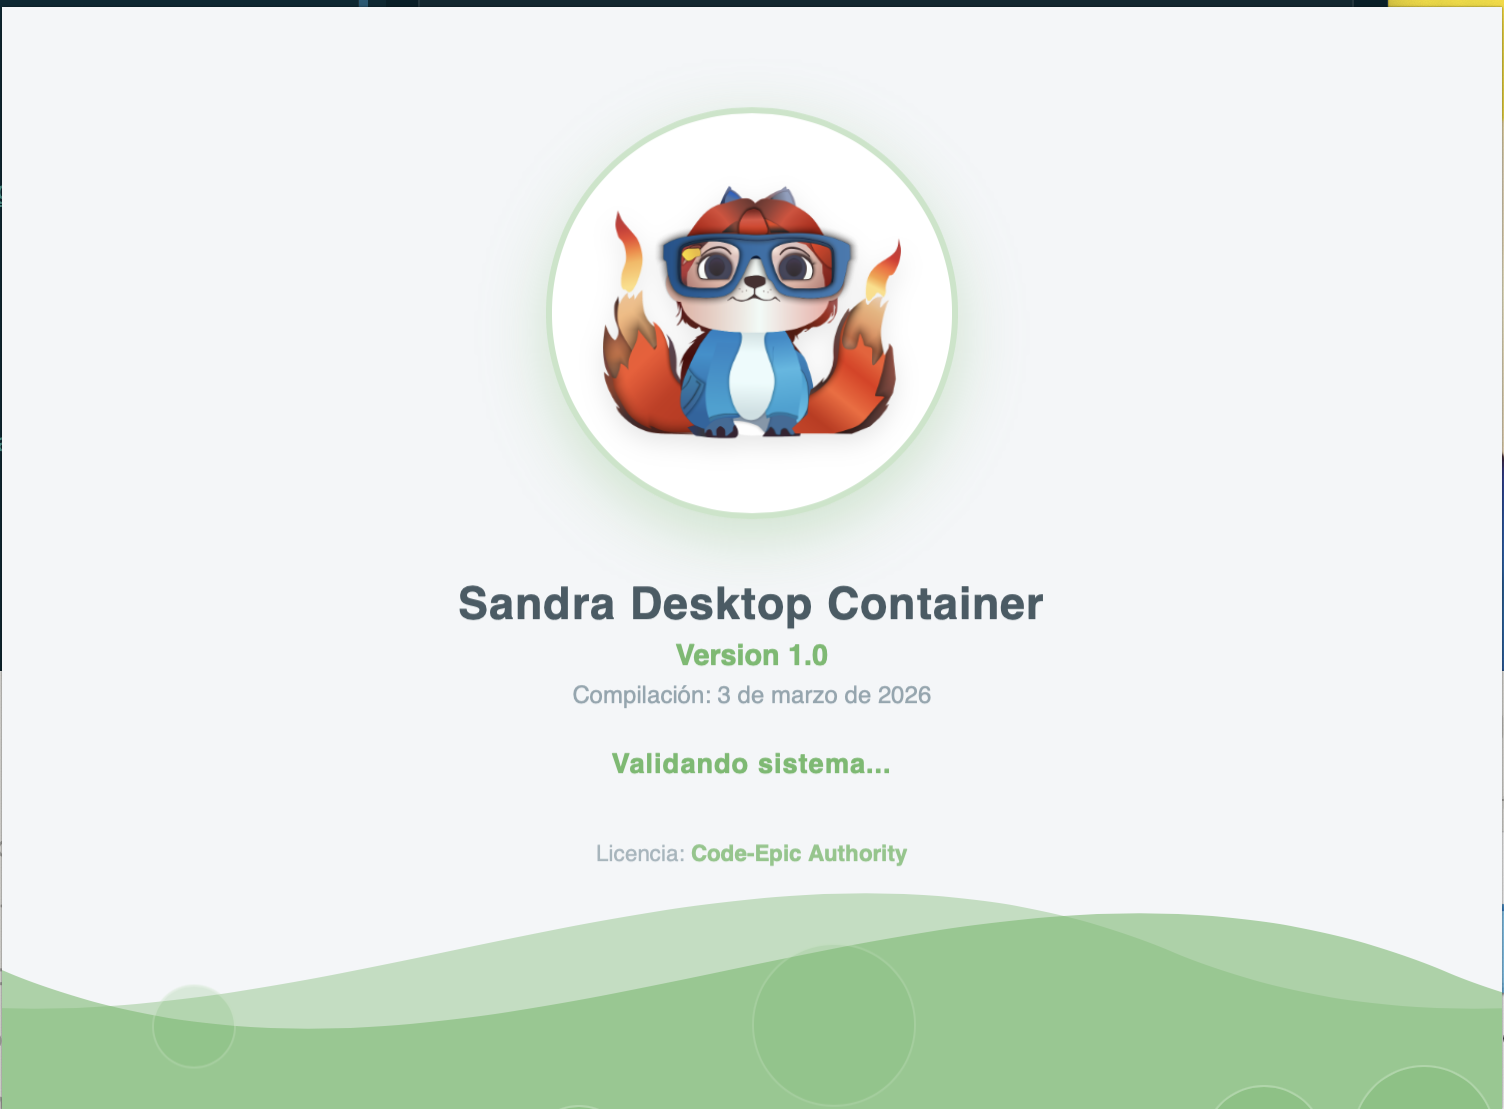
\includegraphics[width=0.9\textwidth]{anexos/1 splash.png}
\caption{Pantalla de bienvenida de SDC}
\label{fig:splash}
\end{figure}

Esta pantalla muestra:
\begin{itemize}[leftmargin=*]
    \item Logo animado de SDC (el mapache con gafas VR)
    \item Version actual del software
    \item Indicador de carga de modulos de seguridad
    \item Verificacion de integridad del sistema
\end{itemize}

\begin{quote}
\textbf{Verificacion de Integridad}\\
\small
Durante la pantalla de bienvenida, SDC realiza una verificacion criptografica de todos los modulos del sistema para detectar posibles alteraciones o corrupciones. Si se detecta alguna anomalia, el sistema se bloqueara y mostrara una alerta de seguridad.
\end{quote}

\section{Resumen del Proceso de Onboarding}

El proceso de onboarding completo sigue estos pasos secuenciales:

\begin{enumerate}
    \item \textbf{Inicio}: Lanzamiento de la aplicacion SDC
    \item \textbf{Configurar Identidad}: Introducir nombre de equipo y area
    \item \textbf{Detectar Entorno}: Escaneo automatico del sistema
    \item \textbf{Generar Client ID}: Creacion del identificador unico
    \item \textbf{Verificar Integridad}: Comprobacion de modulos de seguridad
    \item \textbf{Dashboard}: Acceso al panel principal de control
\end{enumerate}

\section{Solucion de Problemas Comunes}

\begin{table}[H]
\centering
\begin{tabular}{p{5cm}p{8cm}}
\toprule
\textbf{Problema} & \textbf{Solucion} \\
\midrule
Nombre de equipo duplicado & Agregar sufijo numerico o identificador de ubicacion \\
No se detecta IP local & Verificar conexion de red y permisos del sistema \\
Client ID ya existe & Contactar administrador para desvincular dispositivo anterior \\
Error de verificacion & Reiniciar aplicacion; si persiste, reinstalar SDC \\
\bottomrule
\end{tabular}
\caption{Problemas comunes durante el onboarding}
\label{tab:problemas-onboarding}
\end{table}
